\documentclass[aspectratio=169]{beamer}
\usetheme{Madrid}
\usecolortheme{beaver}
\usepackage[utf8]{inputenc}
\usepackage[T1]{fontenc}
\usepackage{tikz}
\usepackage{amssymb}
\usepackage{graphicx}
\setbeamertemplate{navigation symbols}{}
\setbeamercolor{title}{fg=white,bg=cyan!60!black}
\setbeamercolor{frametitle}{fg=white,bg=cyan!50!black}
\setbeamercolor{block title}{bg=cyan!15,fg=black}
\setbeamercolor{block body}{bg=cyan!5,fg=black}

\title{G6 — Collision \& Physics}
\subtitle{Hitboxes, bouncing, gravity, knockback}
\author{ByteForge --- Grade 7 --- Game Maker --- Week Overview}
\date{}

\begin{document}

\begin{frame}
    \titlepage
\end{frame}

\begin{frame}{This Week's Plan}
    \begin{itemize}
        \item Lesson 1: Hitbox Check
        \item Lesson 2: Bounce \& Gravity
        \item Lesson 3: Knockback
        \item[$\bigstar$] BOSS --- Breakout Clone (\texttt{lessonBoss.tex})
    \end{itemize}
\end{frame}

\begin{frame}{Real-World Example}
    \Large
    A basketball's arc and bounce follows the exact same idea — gravity constantly pulling it down (velocity increasing each moment) until it hits the floor and reverses. Minecraft has real block physics too — sand and gravel actually fall when unsupported, using this exact gravity-as-a-loop idea (just without the bounce).
\end{frame}


\begin{frame}{Image}
    \begin{center}
    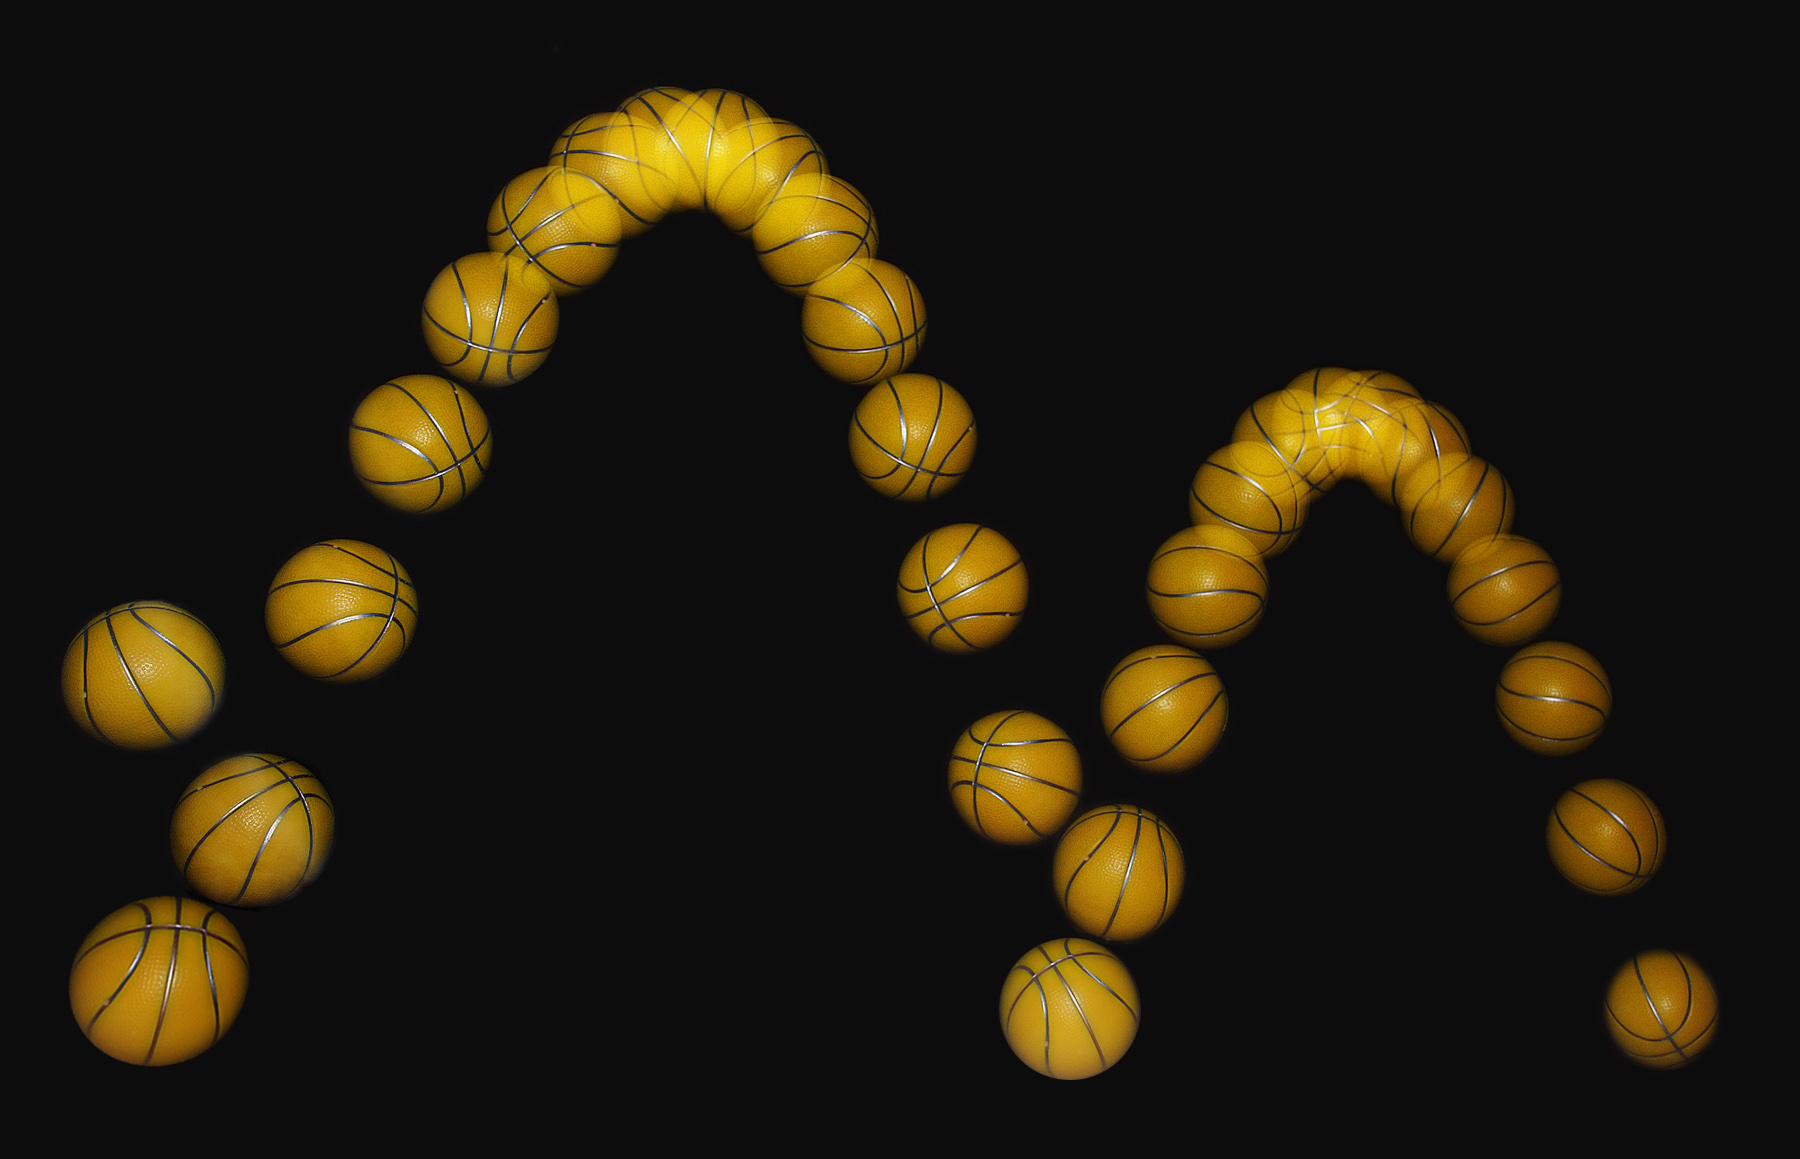
\includegraphics[width=0.55\textwidth]{../images/bounce.jpg}

    \small Bouncing ball strobe photo — MichaelMaggs / Richard Bartz, CC BY-SA 3.0, via Wikimedia Commons
    \end{center}
\end{frame}

\begin{frame}{Let Them Discover}
    \Large
    Drop a ball (real or a video of one bouncing) and watch closely: does each bounce go exactly as high as the last, or does it lose a little height each time? What in the code (Bounce \& Gravity) causes that?
\end{frame}

\begin{frame}{Files in This Folder}
    \small
    \begin{itemize}
        \item \texttt{lesson1.tex} --- Hitbox Check
        \item \texttt{lesson2.tex} --- Bounce \& Gravity
        \item \texttt{lesson3.tex} --- Knockback
        \item \texttt{lessonBoss.tex} --- BOSS: Breakout Clone
    \end{itemize}
    \vspace{0.5em}
    \normalsize Each lesson file is its own short deck --- open the one for
    the specific day you're teaching, not this whole overview.
\end{frame}

\end{document}
